% THIS IS SIGPROC-SP.TEX - VERSION 3.1
% WORKS WITH V3.2SP OF ACM_PROC_ARTICLE-SP.CLS
% APRIL 2009
%
% It is an example file showing how to use the 'acm_proc_article-sp.cls' V3.2SP
% LaTeX2e document class file for Conference Proceedings submissions.
% ----------------------------------------------------------------------------------------------------------------
% This .tex file (and associated .cls V3.2SP) *DOES NOT* produce:
%       1) The Permission Statement
%       2) The Conference (location) Info information
%       3) The Copyright Line with ACM data
%       4) Page numbering
% ---------------------------------------------------------------------------------------------------------------
% It is an example which *does* use the .bib file (from which the .bbl file
% is produced).
% REMEMBER HOWEVER: After having produced the .bbl file,
% and prior to final submission,
% you need to 'insert'  your .bbl file into your source .tex file so as to provide
% ONE 'self-contained' source file.
%
% Questions regarding SIGS should be sent to
% Adrienne Griscti ---> griscti@acm.org
%
% Questions/suggestions regarding the guidelines, .tex and .cls files, etc. to
% Gerald Murray ---> murray@hq.acm.org
%
% For tracking purposes - this is V3.1SP - APRIL 2009

\documentclass{acm_proc_article-sp}
\usepackage{color}
\usepackage{hyperref}

\newcommand{\jeff}[1]{\textcolor{red}{\textbf{Jeff:} #1}}
\newcommand{\john}[1]{\textcolor{blue}{\textbf{John:} #1}}

\begin{document}

\title{Benchmarking In-Memory Streaming Database Management Systems\thanks{Code Here: \url{github.com/jmeehan16/streambench}}}
\subtitle{[Extended Abstract]}
%
% You need the command \numberofauthors to handle the 'placement
% and alignment' of the authors beneath the title.
%
% For aesthetic reasons, we recommend 'three authors at a time'
% i.e. three 'name/affiliation blocks' be placed beneath the title.
%
% NOTE: You are NOT restricted in how many 'rows' of
% "name/affiliations" may appear. We just ask that you restrict
% the number of 'columns' to three.
%
% Because of the available 'opening page real-estate'
% we ask you to refrain from putting more than six authors
% (two rows with three columns) beneath the article title.
% More than six makes the first-page appear very cluttered indeed.
%
% Use the \alignauthor commands to handle the names
% and affiliations for an 'aesthetic maximum' of six authors.
% Add names, affiliations, addresses for
% the seventh etc. author(s) as the argument for the
% \additionalauthors command.
% These 'additional authors' will be output/set for you
% without further effort on your part as the last section in
% the body of your article BEFORE References or any Appendices.

\numberofauthors{2} %  in this sample file, there are a *total*
% of EIGHT authors. SIX appear on the 'first-page' (for formatting
% reasons) and the remaining two appear in the \additionalauthors section.
%
\author{
% You can go ahead and credit any number of authors here,
% e.g. one 'row of three' or two rows (consisting of one row of three
% and a second row of one, two or three).
%
% The command \alignauthor (no curly braces needed) should
% precede each author name, affiliation/snail-mail address and
% e-mail address. Additionally, tag each line of
% affiliation/address with \affaddr, and tag the
% e-mail address with \email.
%
% 1st. author
\alignauthor
John Meehan \\
john@cs.brown.edu
\alignauthor
Jeff Rasley \\
jeffra@cs.brown.edu
}
% Just remember to make sure that the TOTAL number of authors
% is the number that will appear on the first page PLUS the
% number that will appear in the \additionalauthors section.

\maketitle
\begin{abstract}
In this paper, we compare the modern distributed main-memory streaming system Spark Streaming to a major competitor in the commercial space.  We analyze the throughput and latency of the two systems under a variety of conditions and workloads, and in both the distributed and non-distributed space.  We provide an unbiased comparison and detail our methodologies in order to encourage future benchmarking efforts.
\end{abstract}

% A category with the (minimum) three required fields
\category{H.2.4}{Database Management}{Streaming, Benchmarking}

\terms{Database Management, Streaming, Benchmarking}

\section{Introduction}
This is the super-awesome intro section that talks about our
whole project yo!

\section{Background}
\subsection{Streaming Overview}
In a traditional database management system, data is imported into a relatively static data structure.  A user is able to run any queries necessary in order to retrieve desired information.  Streaming systems take the opposite approach, percieving the data as consistently changing.  Continuous queries are written into the system in order to perform analytics on this flow of information, particularly on a subsection, or window, of time.

For instance, say that a stock broker wishes to purchase a particular stock when a five-minute moving average crosses a particular threshold.  In this case, the incoming ticker price for this stock is the stream of information, a sliding window of five minutes is placed on this stream, and a continuous query aggregates this data to calculate the average.  A filter operator is placed further downstream of the window in order to trigger further operators if the threshold is met.

\subsection{Modern Streaming Systems}
Due to the nature of real-time processing, it is crucial that all processing take place in memory with minimal requests to disk.  Therefore it is not surprising that distributed, main-memory database systems have become the key players in the streaming database research space.  These systems take advantage of the fact that many streaming applications are highly parallizeable in order to distribute the stream processing across multiple worker machines.  In this paper, we compare the popular distributed system, Spark Streaming, to an established commercial system, which we will call this "System-X."

\subsubsection{Spark Streaming}
Spark Streaming builds on Apache Spark, creating a streaming API on top of the existing main-memory distributed system.  Also known as Discretized Streams, this system takes advantage of Spark's resilient NOTE LOOK UP RDDs in order to store streaming state.~\cite{dstreams}  Time intervals are discretized in order to allow Spark to batch all information within a specific interval, similar to Jennifer Widom's CQL. NOTE SITE CQL  Intermediate states are stored in the system, in order to easily calculate windows and compute aggregates.  Applications for Spark are programmed using Scala syntax, and make heavy use of map reduce operations to parallelize its processing.

\subsubsection{System-X} 
System-X is an established streaming system, built on research which helped to define streaming systems at their inception.  It is primarily designed to be highly user-friendly, providing methods to interface with a large number of applications.  System-X makes use of a graphical programming user interface, but also provides its own "Streaming SQL" language.
\section{Methodology}

\subsection{Strategy}
\label{ssec:strategy}
Streaming systems are typically evaluated by two major metrics:
\begin{itemize}
\item \textbf{Throughput:} We evaluate throughput as the number of tuples that a full system is capable of processing per second.
\item \textbf{Latency:} We consider latency numbers to be the period of time between a tuple's generation and when it is fully processed by the streaming system.  The latency number that a window reports each reporting interval is the current time minus the timestamp of its oldest tuple.
\end{itemize}

\subsection{Tuple Generation}
\label{ssec:tuple-gen-meth}
In both of the benchmarks we use in our comparisons, we consider a tuple to be string of text of a fixed number of words, the first of which indicates the tuple's epoch timestamp in milliseconds.  We then append a second timestamp to the tuple at the end of processing.  We calculate our latency by subtracking our initial timestamp from our final timestamp.  We calculate our throughput by counting the number of tuples with an initial timestamp that are processed within the given window of time.

\subsection{Architecture Philosophy}
\label{ssec:arch-phil}
A typical streaming system receives new tuples of data from an outside source via some external connection.  The system then processes the data, stores information as necessary, and then outputs results as another stream to be displayed or used by other applications.  In this work, we are only interested in evaluating the stream processing portion of this process.

When benchmarking specific workloads, we intended to put as little external strain on the system as possible in order to avoid contaminating our results.  The actual streaming system is hosted on a specific number of machines, with separate machines generating tuples and sending them via the network.  In addition, the output is also sent to yet another machine and written to disk there, again minimizing extra strain on the machines actually performing the workload.

\subsection{Benchmarks}

\begin{figure}[b]
\centering
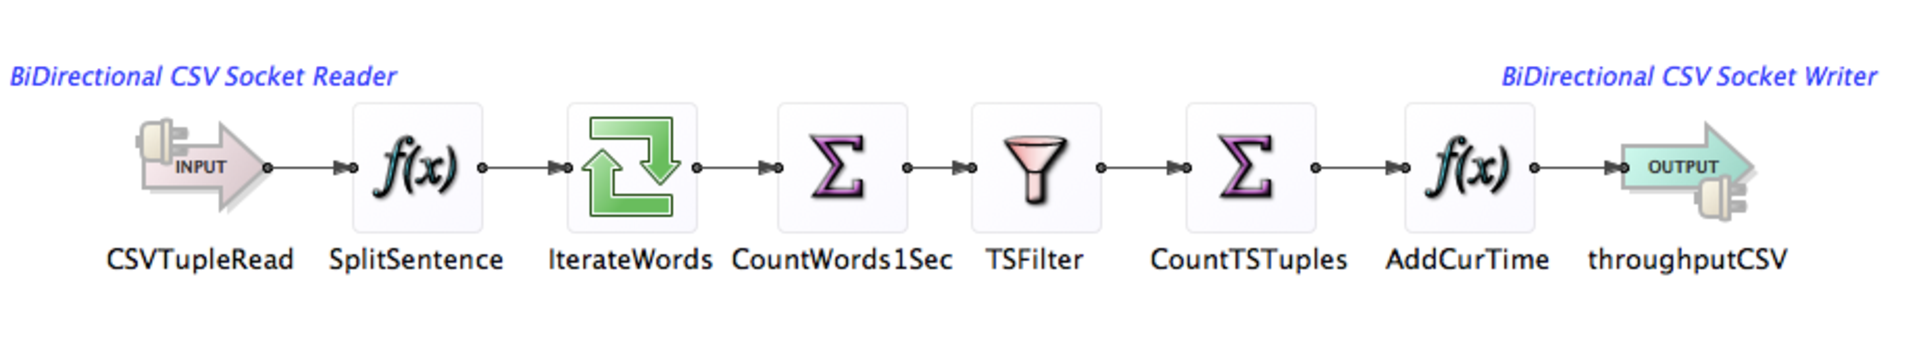
\includegraphics[width=1\linewidth]{figures/System-XWorkflow.pdf}
%\vspace{5.3in}
\caption{Graphical representation of the Wordcount benchmark in System-X}
\label{fig:wordcount}
\end{figure}

We evaluated our systems using two workloads: Wordcount and Grep

\subsubsection{Wordcount}
In the Wordcount benchmark, each input tuple is broken down into individual words and counted within a window of time.  This benchmark should favor Spark, as it is highly parallelizeable.   Spark breaks these tuples into an array of words and then performs map and reduce operations to find their counts.  System-X on the other hand must iterate over each tuple, generate a new tuple for each word, and then perform an aggregation on the resulting tuples.

\subsubsection{Grep}
In the Grep benchmark, input tuples are sent through a filter operation in order to find sentences which contain the word ``the''.  Both Spark and System-X execute similar strategies for this benchmark.

\begin{figure}[t]
\centering
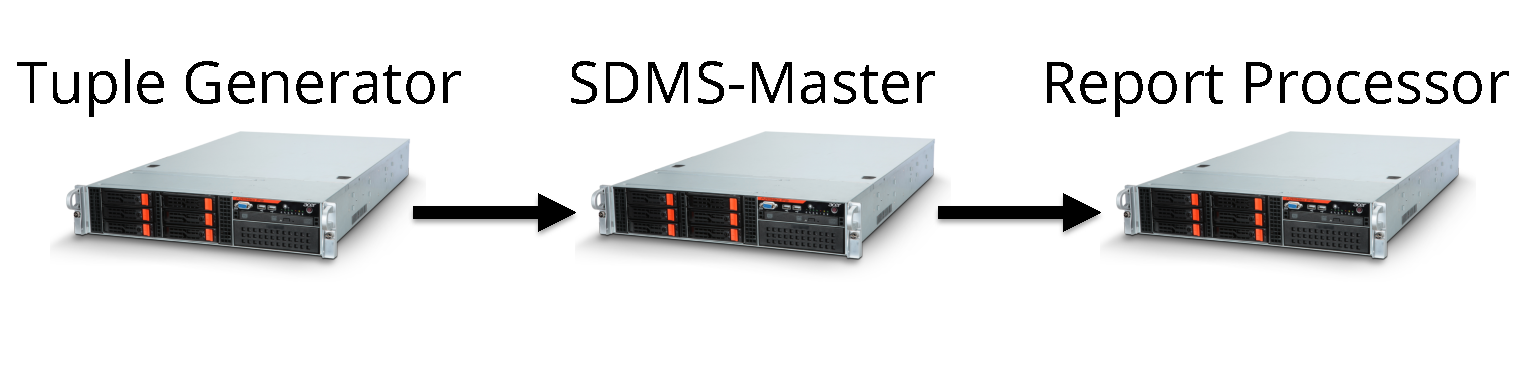
\includegraphics[width=1\linewidth]{figures/diagram.pdf}
%\vspace{-0.3in}
\caption{Single-node cluster setup for benchmarking}
\label{fig:sb1-tput}
\end{figure}

\begin{figure}[b]
\centering
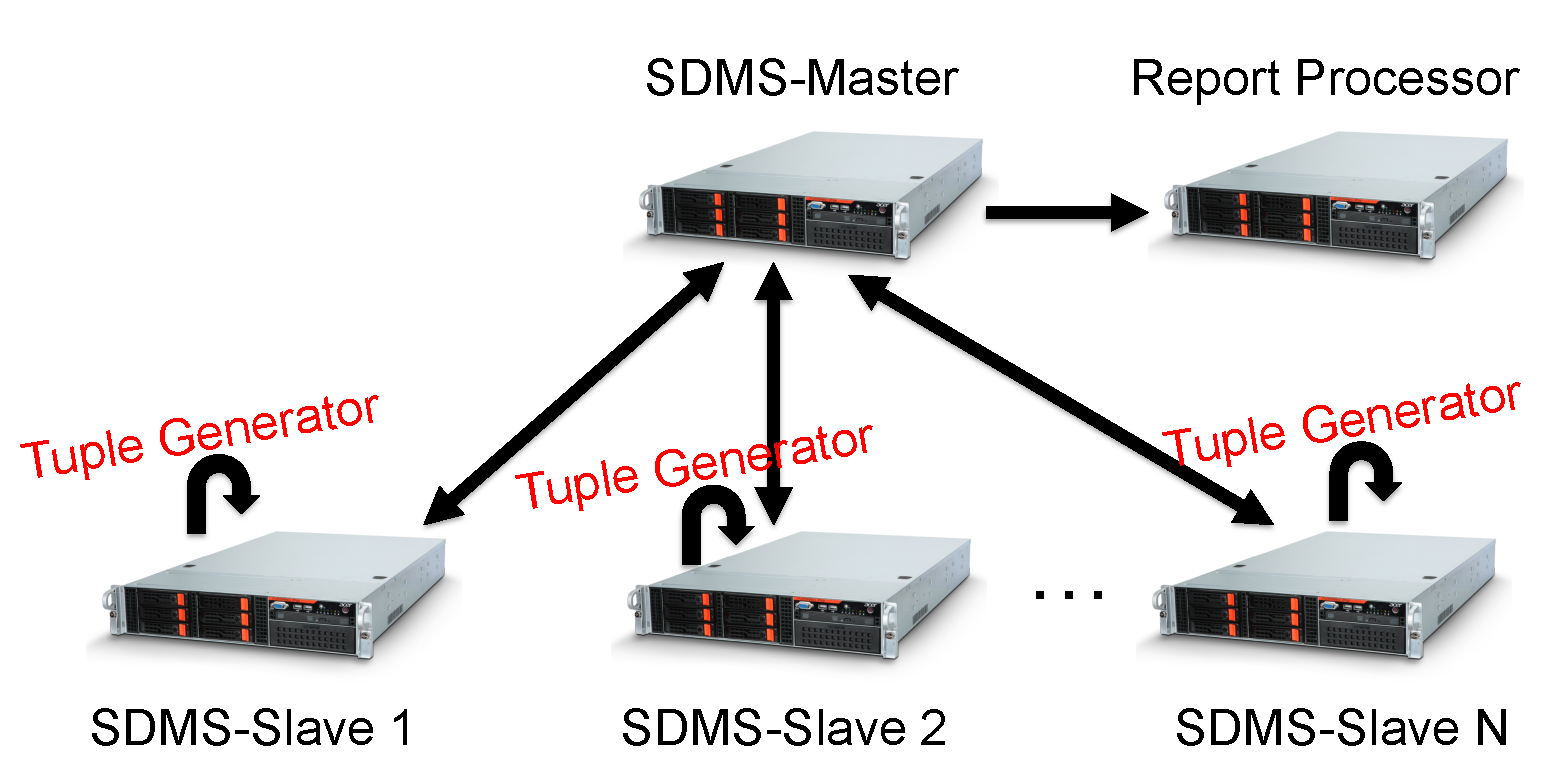
\includegraphics[width=1\linewidth]{figures/spark-full-diagram.pdf}
%\vspace{-0.3in}
\caption{Multi-node cluster setup for benchmarking Spark}
\label{fig:sb1-tput}
\end{figure}




\section{Implementation}
This section details the implementation of our benchmarking system.
\subsection{Cluster}
As mentioned in section \john{put the methodology section here}, the ideal cluster for a Spark system involves one master machine, X worker nodes, X tuple generators, and a node to collect output.  Previous benchmarking attempts have been performed on Amazon's EC2 machines.  This provides the advantage of having an elastically-sized cluster that can easily be set up and replicated.  The disadvantage of using EC2 machines, however, is that each node is a virtual machine that may not be receiving the resources that are expected.  Additionally, there is little to no control over the network bandwidth on these machines, or what other information might be affecting throughput.  For these reasons, we chose to build our own cluster instead.  This was later determined to be a mistake (see Section \john{regrets section here}).

Our cluster was limited to four AMD Athlon(tm) 64 X2 Dual Core Processor 3800+ machines, each with 3GB of memory and 2 core, 2Ghz processors.  For our single-node experiments, tuple generation and collection were performed on separate nodes from the actual benchmark in an effort to record more accurate throughput numbers.  However, for Spark clusters of size 2 or more, the tuple generators were run on the same machines as the worker nodes due to a lack of machines.

\subsection{Tuple Generator}
As mentioned in section \john{tuple generation section}, tuples are defined as a timestamp followed by a sentence of variable number of words.  Generating these tuples is a two-fold process.  First, a sample file of sentences of a specified word count is pre-generated using a python script.  By generating this file ahead of time, we are able to normalize the input sent to both Spark and System-X.

A second python script then processes our sample file of sentences.  This script prepends a timestamp to the string as the first word.  The timestamp includes of "TS-" in order to distinguish the timestamp from the other words.  The tuples are then sent to the streaming application at a throughput rate specified as an input parameter.  The throughput rate starts small, and gradually increases until the streaming application is saturated and eventually fails.

Initially, the throughput rate on our tuple generator program was simply controlled using the Thread.sleep command.  However, it was discovered that this method is not granular enough to generate tuples at a high enough rate to consistently saturate our systems.  The reason for this is that Thread.sleep is unreliable beyond approximately a 0.1 ms waittime.  This means that the maximum throughput of our generator was about 10,000 tuples.

Our solution to this problem was to add a second factor, a batch size for tuples.  To generate a higher throughput, we choose to send a batch of tuples, then wait for a specified amount of time, then send the next batch, and so on.  The equation used to calculate the optimal wait time and batch size is:

\john{equation goes here}

We determined what our batch size should be using the following equation:

\john{equation goes here}

By plugging the result for {b} into the first equation, we are able to calculate the optimal wait time to generate the desired throughput.

\subsection{Performance Analysis}
In our original implementation, none of the performance analysis was performed within the streaming system.  Instead, the Wordcount or Grep output was sent to a separate machine, where it would be written to a file and analyzed by a separate script.  This script would calculate throughput and latency numbers by comparing the timestamps within the sentence tuples to the timestamps attached by the streaming system.  While this method did not require additional processing by the system, we found that the act of printing so much information to the TCP output stream was negatively affecting our performance.  We determined that it would be more fair to instead perform the aggregate within the streaming system itself, and only output this number.

In the Wordcount benchmark, after the words have been counted for a given window, the "TS-" timestamp words are filtered, and their respective counts are summed in order to determine the throughput.  The minimum timestamp from that window is then subtracted from the current timestamp in order to calculate the latency.

In the Grep benchmark, it was impossible to calculate throughput numbers after the grep count (number of sentences with the word "the") had been determined.  This is because some tuples had been filtered, but should be counted towards throughput.  Instead, we simply branch the throughput and latency calculations from the source of the stream, giving us accurate numbers for all input tuples.
\section{Challenges}
These are our challenges..

\section{Results}
Results!

\begin{figure}[t]
\centering
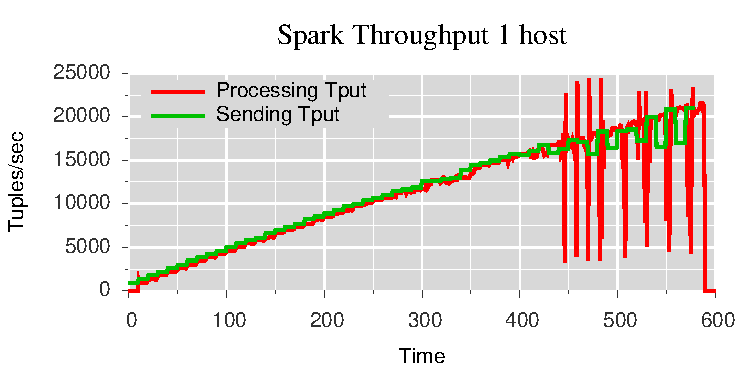
\includegraphics[width=1\linewidth]{figures/sp1_tput.pdf}
%\vspace{-0.3in}
\caption{Throughput/Time for a single Spark host. We sent 1KB tuples at a slowly ramped up rate from 1K tuples/sec to 30k tuples/sec with a step size of 500 tuples/sec. The sending rate remained constant for 10 seconds before transitioning to the next throughput.}
\label{fig:sb1-tput}
\end{figure}

\begin{figure}[t]
\centering
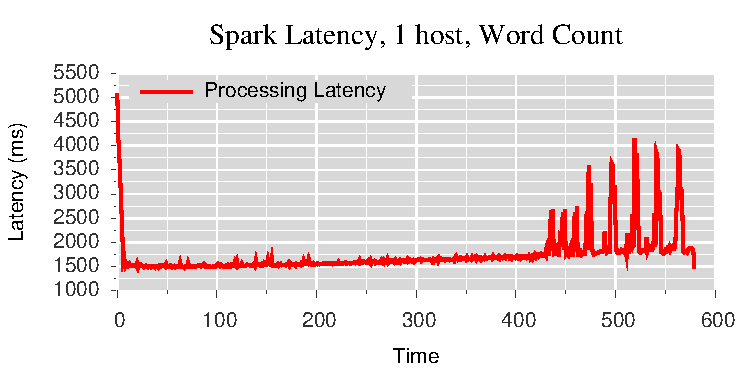
\includegraphics[width=1\linewidth]{figures/sp1_latency.pdf}
%\vspace{-0.3in}
\caption{Average latency to process tuples for a single Spark host. Similar to Figure~\ref{sb1-tput} we sent 1KB tuples at a slowly ramped up rate from 1K tuples/sec to 30k tuples/sec with a step size of 500 tuples/sec. The sending rate remained constant for 10 seconds before transitioning to the next throughput. The astute reader will notice that the latency spike in this graph occurs at the same time as the loss in throughput consistency in Figure~\ref{sb1-tput}}
\label{fig:label-me-if-you-want}
\end{figure}


\section{Lessons Learned}
\label{sec:lessons}
During this project, a number of decisions were made that cost the authors a significant amount of time.  If given the opportunity to revisit this project, here is what we would do differently.

\subsection{EC2}
As mentioned in section~\ref{sec:impl}, we chose not to use an EC2 cluster for our experiments due to concerns about inconsistent resources in the cloud.  In retrospect, this was a mistake.  The flexibility, additional resources, and ease of setup make EC2 the obvious choice for cluster-based benchmarking needs.  Additional research has also revealed our fears about inconsistent resources were unfounded, as the more expensive EC2 instances provide predictable performance.

\subsection{Tuple Generation}
When generating tuples, it is necessary to be able to control the number of tuples being produced per second.  We chose to create each tuple as a discrete unit, using Thread.sleep to control the total number of tuples being sent.  The problem with this strategy is that Thread.sleep is documented at being able to sleep for a minimum time of 7 us before the call to the system clock takes longer than the actual sleep time.  In practice, however, we found that Python's sleep call has a minimum sleep time of 100 us, meaning that we were only able to generate 10,000 tuples per second without using other flow control methods.

Sending raw bytes rather than text-based tuples would have been a better strategy, particularly for Spark.  Spark contains a "RateLimitedStream" object, which can generate a stream of data with a limit on the number of bytes per second.  This is an ideal benchmarking tool.  System-X, however, expects tuples to be sent, and thus would have needed to convert the bytes into tuples before processing them.

\subsection{Socket Bottlenecks}
Our tuple generator was designed with the false assumption that it would reliably generate tuples at the specified rate.  If this were the case, then whenever the system became backlogged, throughput output from the system would remain constant, while the throughput output from the generator would continue increasing.  In addition, an increase in latency would be visible when the system is saturated.

Instead, we found that once the TCP socket buffer is full on the receiver's side, it signals the sender program to stop sending new tuples.  Effectively, this freezes our tuple generator program for a very short period of time, allowing the streaming system to catch up.  As a result of this misunderstanding, calculating the maximum throughput of the system was much more difficult than expected.  We instead ended up using the strategy outlined in section \john{results section}.

\subsection{System-X Unicode}
System-X does not support unicode by default, and does not fail gracefully.  Instead, it will continuously attempt to process the same tuple, but will never actually succeed which actually causes the entire system to crash. We are considering filing an official bug with the makers of System-X since this is a horrible DoS security bug if untrusted tuples were coming into your system.

\subsection{System-X distributed}
\label{ssec:sysx-dist}
System-X is advertised as being "distributed system ready."  While this is technically true, there is no method of automating the creation of a distributed workflow, and it must instead be built manually.  Due to licensing issues and time constraints, we were unable to complete a working distributed workflow for System-X for this paper.


\section{Acknowledgments}
Thank you.

%
% The following two commands are all you need in the
% initial runs of your .tex file to
% produce the bibliography for the citations in your paper.
\bibliographystyle{abbrv}
\bibliography{bibdata}  % sigproc.bib is the name of the Bibliography in this case
% You must have a proper ".bib" file
%  and remember to run:
% latex bibtex latex latex
% to resolve all references
%
% ACM needs 'a single self-contained file'!
%
%APPENDICES are optional
%\balancecolumns
%\appendix
%Appendix A

\balancecolumns
% That's all folks!
\end{document}
